% Clean CV/Resume Template, by Bennet B <dev@bennet.cc>
% CC0, Public-Domain
% 
% Permission is hereby granted, free of charge, to any person obtaining a copy
% of this template and associated files (the "Template"), to deal
% in the Template without restriction, including without limitation the rights
% to use, copy, modify, merge, publish, distribute, sublicense, and/or sell
% copies of the Template, and to permit persons to whom the Template is
% furnished to do so, subject to the following conditions:
%
% The above copyright notice and this permission notice shall be included in all
% copies or substantial portions of the Template.
%
% THE TEMPLATE IS PROVIDED "AS IS", WITHOUT WARRANTY OF ANY KIND, EXPRESS OR
% IMPLIED, INCLUDING BUT NOT LIMITED TO THE WARRANTIES OF MERCHANTABILITY,
% FITNESS FOR A PARTICULAR PURPOSE AND NONINFRINGEMENT. IN NO EVENT SHALL THE
% AUTHORS OR COPYRIGHT HOLDERS BE LIABLE FOR ANY CLAIM, DAMAGES OR OTHER
% LIABILITY, WHETHER IN AN ACTION OF CONTRACT, TORT OR OTHERWISE, ARISING FROM,
% OUT OF OR IN CONNECTION WITH THE TEMPLATE OR THE USE OR OTHER DEALINGS IN THE
% TEMPLATE.
%
% based on Modern CV by Habib Semouma
% https://www.overleaf.com/latex/templates/modern-cv-slash-resume-template/vjrqdkpjckwj
%
% 
\documentclass[oneside]{article}

\usepackage{wallpaper}
\usepackage{geometry}
\usepackage[
    unicode=true,
    bookmarks=true,
    bookmarksnumbered=false,
    bookmarksopen=true,
    bookmarksopenlevel=1,
    breaklinks=false,
    pdfborder={0 0 0},
    backref=false,
    colorlinks=false
    ]{hyperref}
\usepackage{lastpage}
\usepackage{hyphenat}
\usepackage{hyphsubst}
\usepackage{tabularx}
\usepackage{moresize}
\usepackage[document]{ragged2e}
% \usepackage{parskip}

\usepackage[scaled]{helvet}
\usepackage{fontawesome5}
\usepackage[defaultfam,tabular,oldstyle]{montserrat}
\usepackage[T1]{fontenc}
\renewcommand*\oldstylenums[1]{{\fontfamily{Montserrat-TOsF}\selectfont #1}}

\usepackage{titlesec}
\usepackage{xcolor}
\usepackage{tikz}

\setlength{\parindent}{0pt}
\titleformat{\section}{\normalfont}{}{0pt}{}

\renewcommand{\arraystretch}{1.4}

\setlength\fboxrule{0pt}
\setlength\fboxsep{12pt}
% \setlength{\parskip}{.5\baselineskip plus 2pt}
% \renewcommand{\baselinestretch}{1.1}

\titlespacing{\section}{0pt}{1.5ex plus .1ex minus .2ex}{1pc}

\newcolumntype{Y}{>{\RaggedRight\arraybackslash}X}

% Change PDF Meta Info here
\hypersetup{
    pdftitle={Jahanvi - CV - English},
    pdfauthor={Jahanvi},
    pdfsubject={CV}
}

% Paper size
\geometry{
    a4paper,
    left=0pt,
    right=0pt,
    top=0pt,
    bottom=0pt,
    nohead,
    % includefoot,
    nomarginpar
}

% Background Color of the Sidebar Column
\definecolor{sidebg}{cmyk}{1, 0.02, 0, 0.56}
% Background Color of the Main Column
\definecolor{mainbg}{cmyk}{0, 0, 0.07, 0.04}

% Text Color of the Main Column
\definecolor{maintext}{cmyk}{1, 0.02, 0, 0.8}
% Text Color of the Sidebar Column
\definecolor{sidetext}{cmyk}{0, 0, 0.07, 0.04}

\pagecolor{mainbg}

\begin{document}
\setlength{\topskip}{0pt}\setlength{\footskip}{0pt}%
\fcolorbox{red}{sidebg}{%
    \begin{minipage}[t][\textheight-2\fboxsep-2\fboxrule][t]{\dimexpr0.40\textwidth-2\fboxrule-2\fboxsep\relax}
        \color{sidetext}
        %%%%%%%%%%%%%%%%%%%%%%%%%%%%%%%%%%%%%%%%%%%%%%%%%%%%
        % YOUR NAME, PRONOUNS, OCCUPATION(s), AND HEADSHOT

      \vspace*{0cm}

      \begin{center}
       {\bfseries\scshape\HUGE Jahanvi }
      \end{center}

       \vspace{0cm}
        \\
         \\
        
        \\
     \begin{center}
            \begin{tikzpicture}
            \clip (0,0) circle (3cm) node[anchor=center] {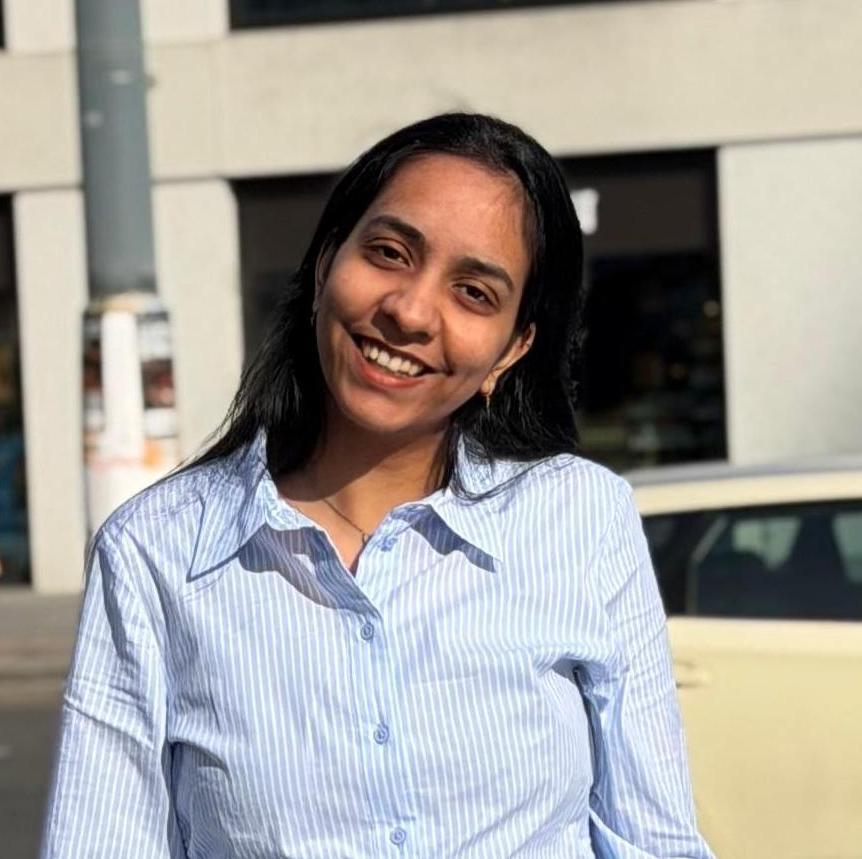
\includegraphics[width=6cm]{jaanii.jpg}}; 
            \end{tikzpicture}
        \end{center}
        \vspace{0cm}
        %%%%%%%%%%%%%%%%%%%%%%%%%%%%%%%%%%%%%%%%%%%%%%%%%%%%
        % YOUR PERSONAL INFROMATION
        \phantomsection{}
        \addcontentsline{toc}{section}{Personal info}
        \section*{\large Personal info}
        \begin{tabularx}{\textwidth}{cY}
            \faStarOfLife{} & 21/10/2004 \\
            \faPhone{}      & +49 17622867488 \\
            \faMapMarker{}  & Berlin, Germany\\

        \end{tabularx}
        \vspace{0cm} \\
        \rule{\linewidth}{0.4pt} \\
        %%%%%%%%%%%%%%%%%%%%%%%%%%%%%%%%%%%%%%%%%%%%%%%%%%%%%%%%%
        % YOUR LINKS, YOU MAY ALSO ADD A PERSONAL WEBSITE OR PORTFOLIO
        \phantomsection{}
        \addcontentsline{toc}{section}{Links}
        \section*{\large Links}
        \begin{tabular}{cl}
        %    \faCode{}     & \href{https://example.com}{example.com}
            \faGithub{}   & \href{https://github.com/jaanii-code}{/jaanii-code} \\
            \faLinkedin{} & \href{https://www.linkedin.com/in/jahanvi-verma-713ba0354/}{/jahanvi-verma-713ba0354} \\
        \end{tabular}
        \vspace{0.2cm} \\
        \rule{\linewidth}{0.4pt} \\

         %%%%%%%%%%%%%%%%%%%%%%%%%%%%%%%%%%%%%%%%%%%%%%%%%%%%%%%%%%%%
        % YOUR SKILLS
        % Add/Remove as seen fit, Icons: https://packages.oth-regensburg.de/ctan/fonts/fontawesome5/doc/fontawesome5.pdf
        \phantomsection{}
        \addcontentsline{toc}{section}{Skills}
        \section*{\large Skills}
        \vspace*{-0.2cm}
        \begin{tabularx}{\textwidth}{cY}
       
    \faCode{} &
   {C++},
    {C},
    {Python},
    {PHP},
    {JavaScript},
    {C\#},
    {Java},
    {Database},
    {MySQL},
    {Data Structures and Algorithms}
    {Object-Oriented Programming}
    \\

    \faPen*{} &
    \textcolor{yellow}{\LaTeX},
    \textcolor{yellow}{HTML},
    \textcolor{yellow}{CSS} \\

    \faFont{} &
    \textcolor{white}{{MS Office, GSuite, Adobe Acrobat}} \\

    \faCogs{} &
    \textcolor{pink}{Windows, macOS} \\
    \faUsers{} &
     \textcolor{white}{{TeamWork, Time-Management, Critical Thinking,  Problem Solving,  Logical Thinking, Communication skils, Adapatability, creativity}} \\

\end{tabularx}
 \vspace{0pt} \\
        \rule{\linewidth}{0.4pt} %%%%%%%%%%%%%%%%%%%%%%%%%%%%%%%%%%%%%%%%%%%%%%%%%%%%%%%%%%
        % LANGUAGES
        \vspace*{-0.3cm}
        \phantomsection
        \addcontentsline{toc}{section}{Languages}
        \section*{\large Languages}
        \begin{tabular}{cl}
            \faLanguage{} & English - Advanced(C1) \\
            \faLanguage{} & German - Elementary (A2) 
        \end{tabular}
        \vspace{0.2cm}
        \\
        \rule{\linewidth}{0.4pt}
        \\%%%%%%%%%%%%%%%%%%%%%%%%%%%%%%%%%%%%%%%%%%%%%%%%%%%%%%%%%%
        % Certificate
      \phantomsection
\addcontentsline{toc}{section}{Certificates}
\section*{\large Certificates}
{\scshape\fontseries{light}\selectfont\footnotesize BSG College of IT}
\begin{itemize}
    \setlength{\itemsep}{-2pt}

    \item Object-Oriented Programming in C
    \item C++ Programming
    \item Python Programming
    \item JavaScript Fundamentals

\end{itemize}

\vspace{-0.1cm}
\rule{\linewidth}{0.4pt}

        
        %%%%%%%%%%%%%%%%%%%%%%%%%%%%%%%%%%%%%%%%%%%%%%%%%%%%%%%%%%%%%%%%
        % GRADESCALE (if nesseary, e.g. if you apply abroad, where scales 
        % are different. You should at least provide, what the best possible
        % grade and what the worst possible grade is)
        \vfill
       
    \end{minipage}
}
\hfill
\fcolorbox{red}{mainbg}{%
    \begin{minipage}[t][\dimexpr\textheight-2\fboxrule-2\fboxsep\relax][t]{\dimexpr0.6\textwidth-2\fboxrule-2\fboxsep\relax}
        \color{maintext}
        %%%%%%%%%%%%%%%%%%%%%%%%%%%%%%%%%%%%%%%%%%%%%%%%%%%%%%%%%%
% PROFILE SECTION
 \vspace*{0.75cm}
\phantomsection{}
\addcontentsline{toc}{section}{Profile}
\section*{\scshape\Large Profile \rule{\linewidth}{0.4pt}}

Motivated Computer Science student with strong problem-solving skills and knowledge of \textcolor{red}{C++}, \textcolor{red}{Python}, \textcolor{red}{MySQL}, and \textcolor{red}{web technologies}. Passionate about learning new technologies and working in collaborative environments

\vspace{0.5cm}

       
        %%%%%%%%%%%%%%%%%%%%%%%%%%%%%%%%%%%%%%%%%%%%%%%%%%%%%%%%%%
        % WORK EXPERIENCE
        \phantomsection{}
        \addcontentsline{toc}{section}{Work Experience}
        \section*{\scshape\Large Work Experience \rule{\linewidth}{0.4pt}}
%
        {\large \textbf{Flink SE}} \\ 
        {{\fontseries{medium}\selectfont Part-time, Ops-Associate}} \\
        {\scshape\fontseries{light}\selectfont\footnotesize June 2025 \textendash{} April 2026} 
        \begin{itemize}
            \setlength{\itemsep}{-3pt}
    \item Maintained and updated \textcolor{red}{database} like inventory records, ensuring consistency, integrity, and error-free data handling.
    \item Utilized digital tools \textcolor{red}{(spreadsheets and record systems)} for real-time data entry, updates, and reporting.
    \item Optimized workflow under deadlines with strong problem-solving skills.
    \item Worked in a fast-paced environment with attention to detail and prioritization.

        \end{itemize}
%
        {\large \textbf{Alex Institute}} \\
        {{\fontseries{medium}\selectfont IELTS Trainer \& Data Management Assistant}} \\
        {\scshape\fontseries{light}\selectfont\footnotesize Aug 2024\textendash{} Jan 2025} 
        \begin{itemize}
            \setlength{\itemsep}{-3pt}
            \item Conducted IELTS training sessions focusing on reading, writing, listening, and speaking skills.
            \item Managed student records and performance data using \textcolor{red}{digital tools} and \textcolor{red}{spreadsheets}.
            \item Maintained accurate \textcolor{red}{database} of enrollments, progress reports, and assessments.
            \item Assisted in organizing schedules and coordinating academic activities efficiently.
            \end{itemize}
           
%
        %%%%%%%%%%%%%%%%%%%%%%%%%%%%%%%%%%%%%%%%%%%%%%%%%%%%%%%%%%%
        % EDUCATION
        \phantomsection{}
        \addcontentsline{toc}{section}{Education}
        \section*{\scshape\Large Education \rule{\linewidth}{0.4pt}}
%
        {\large \textbf{Bsc Computer Science\\ }} \\
        {{\fontseries{medium}\selectfont Gisma University Of Applied Sciences}} \\
        {\scshape\fontseries{light}\selectfont\footnotesize 
        Dec 2024 \textendash{} Present \qquad Berlin, Germany} \\
        {\footnotesize {Relevant Coursework:} \textcolor{red}{Data Structures}, \textcolor{red}{DBMS}, \textcolor{red}{Operating Systems}, \textcolor{red}{Web Development}} \\ 
        
          {\large \textbf{Senior Secondary }} \\
        {{\fontseries{medium}\selectfont Guru Harkrishan Public School}} \\
        {\scshape\fontseries{light}\selectfont\footnotesize 
       2022\textendash{} 2023 \qquad Sri Ganganagar,India} \\
        {\footnotesize Elective Courses: Chemistry, Physics, Maths} \\
       
 % \\
        \vfill%
        {\hfill\small\fontseries{extralight}  \hfill}
  

        % \vspace{.6cm}
        %%%%%%%%%%%%%%%%%%%%%%%%%%%%%%%%%%%%%%%%%%%%%%%%
        % PROJECTS
        \phantomsection
        \addcontentsline{toc}{section}{Projects}
        \section*{\scshape\Large Projects \rule{\linewidth}{0.4pt}}
        \begin{justify}
        \setlength{\parindent}{0pt}
        {\large \textbf{Pizza Restaurant Website}} \\
        {\scshape\fontseries{light}\selectfont\footnotesize BSG College Of IT \qquad 2024} \\
        {\footnotesize
Developed a responsive restaurant website using
\textcolor{red}{HTML},
\textcolor{red}{CSS}, and
\textcolor{red}{JavaScript}. Created interactive pages including home, menu, and contact sections while improving navigation and user experience.} \\
        
          {\large \textbf{University Management System}} \\
          {\scshape\fontseries{light}\selectfont\footnotesize Gisma University Of Applied Sciences \qquad 2026} \\
{\footnotesize
Built a student record management system using
\textcolor{red}{Python} and
\textcolor{red}{MySQL} for storing, updating, and managing student data efficiently.} \\

       {\large \textbf{Personal Portfolio Website}} \\
         {\scshape\fontseries{light}\selectfont\footnotesize Gisma University Of Applied Sciences \qquad 2026} \\
        {\footnotesize
       Developed a responsive portfolio website using
       \textcolor{red}{HTML},
       \textcolor{red}{CSS}, and
       \textcolor{red}{JavaScript} to showcase projects, skills, and contact information.}
        
       
        \end{justify}
        \vfill%
        {\hfill\small\fontseries{extralight}\hfill}
    \end{minipage}
}
\end{document}

